\documentclass[aps,prb,twocolumn,superscriptaddress]{revtex4-2}
\usepackage{graphicx}  % Required for inserting images
\usepackage{hyperref}  % Required for clickable links
\usepackage{wrapfig}
\usepackage{amsmath}
\usepackage{multirow}

\renewcommand{\thefigure}{\arabic{figure}}

\hypersetup{
    colorlinks=true,
    linkcolor=blue,
    filecolor=magenta,      
    urlcolor=cyan,
}

\begin{document}

\title{Advancements in X-Ray Diffraction and X-Ray Free-Electron Lasers}

\author{Simon Lavoie}
\affiliation{Department of Physics, McGill University}
\date{April 2025}

\begin{abstract}
Due to their nanometer-scale wavelengths, X-rays are well-suited for probing
atomic-scale structures.  This paper discusses the leaps in X-ray source
brilliance made possible by particle accelerator technology, leading to
synchrotron lasers and eventually X-ray free-electron lasers. Further, the
effect such X-ray sources have had on X-ray diffraction (XRD) experiments is
studied, exploringas how techniques such as serial femtosecond crystallography
(SFX) and single-particle imaging (SPI) allows scientists to push the spatial
resolution of crystal structure determination down to the nanometer scale. The
temporal characteristics of these powerful pulses are similarly described to
understand how these facilities push the enveloppe of ultrafast science through
pump-probe experiments allowing for real-time imaging of chemical reactions and
phase transitions which is of significant interest to various fields, including
chemistry, biology, crystallography, and much more. Of course, no technique is
free of technical challenges and limitations, and these too will be explored.
\end{abstract}

\maketitle

\section*{Contents}
\begin{itemize}
    \item \hyperref[sec:intro]{Introduction}
    \item \hyperref[sec:theory]{Theoretical Framework}
    \item \hyperref[sec:experiment]{Experimental Methods}
    \item \hyperref[sec:data]{Data Acquisition and Analysis}
    \item \hyperref[sec:challenges]{Challenges and Future Prospects}
\end{itemize}

\section{Introduction} \label{sec:intro}
X-ray diffraction (XRD) has been instrumental in elucidating atomic structures
since its experimental validation in 1912 by Friedrich, Knipping, and von Laue
\cite{vonLaue1912}. X-ray tubes have been the conventional laboratory source of
such radiation, due to their simple assembly and ease of maintenance. Such tubes
have a very low overall efficiency, however, with most of the energy supplied
to the tube being lost due to heat, and therefore requiring continuous cooling
\cite{pecharsky2005fundamentals}. These sources also have a relatively low
intensity, and emit incoherent light.  \textbf{F}ree-\textbf{E}lectron 
\textbf{L}asers (FELs), introduced by John Madey in the early 70's, operated 
at infrared, visible and ultraviolet wavelengths \cite{OGUndulator}. In 2005,
the \textbf{D}eutsches \textbf{E}lektronen-\textbf{SY}nchrotron's (DESY)
\textbf{F}ree-electron \textbf{LAS}er in \textbf{H}amburg (FLASH), Germany,
became the first facility to produce X-rays using this apparatus, with SLAC's 
\textbf{L}inac \textbf{C}oherent \textbf{L}ight \textbf{S}ource (LCLS) 
following suit with higher energy X-rays in 2009. Various other facilities have 
been constructed around the world since. Such advancements in X-ray 
sources have led to a revolution in X-ray diffraction, allowing for the
determination of protein structures using microcrystals, the emerging field of 
serial femtosecond crystallography (SFX), and the study of ultrafast phenomena
at the atomic scale, such as bond formation and breaking during chemical reactions.


\section{Theoretical Framework} \label{sec:theory}
\subsection{Bragg's Law}
Shortly after Röntgen's discovery of X-rays, Max von Laue suggested that X-rays
could be diffracted by crystals, which Friedrich and Knipping experimentally
confirmed in 1912. The underlying principle was formalized by W. H. Bragg and W.
L. Bragg through:
\begin{equation}\label{eq:bragg}
  2d\sin\theta = n\lambda,
\end{equation}
where $d$ is the regular spacing between the atoms, $\theta$ the angle of
incidence, $n$ an integer, and $\lambda$ the X-ray wavelength \cite{Bragg1913}.
As an X-ray beam incident upon a crystal interacts with the electrons of the
lattice's atoms, it is scattered spherically in all directions. The scattered
X-rays from adjacent atoms interfere constructively and destructively, producing
a diffracted beam. The condition for constructive interference is given by Eq.
\ref{eq:bragg}. That is, when the path difference between two adjacent rays
($2d\sin\theta$) is an integer multiple of the wavelength, the waves will
superimpose in phase, leading to peaks in the diffracted intensity. This
phenomenon is illustrated in Fig. \ref{fig:Laue}.

% BRAGG DIFFRACTION FIGURE
\begin{figure}[!h]
    \centering
    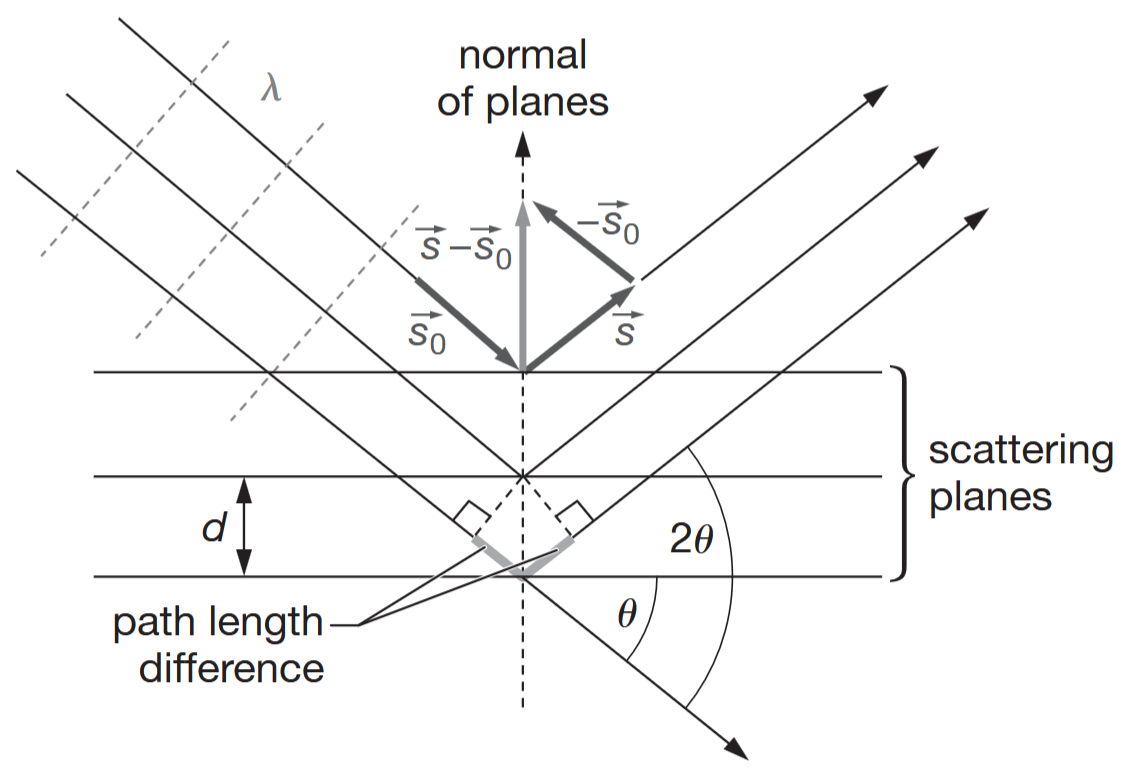
\includegraphics[width=0.9\linewidth]{Figures/Bragg_diffraction_2.svg.png}
    \caption{Geometry of a beam with angle of incidence $\theta$ approaching from the left
    into a symmetrical arrangement of atoms forming the lattice of a crystal \cite{Girolami}. }
    \label{fig:Bragg}
\end{figure}

% LAUE DIFFRACTION PATTERN
\begin{figure}[h]
    \centering
    \includegraphics[width=0.9\linewidth]{Figures/Interferenz-Erscheinungen_bei_Röntgenstrahlen_Tafel_II_Fig._5.jpg}
    \caption{X-ray diffraction pattern of a copper sulfate crystal from
    Friedrich and Knipping's 1912 paper \cite{vonLaue1912}.} \label{fig:Laue}
\end{figure}

\subsection{The Structure of Crystals}
The theory of crystals and how they are structured is essential to understanding
X-ray diffraction. Crystals are regular arrangements of atoms in three
dimensions, exhibiting translational symmetry. The discrete points at which the
atoms of a crystal are located can be described mathematically by 
\begin{equation}\label{eq:lattice}
    \mathbf{R} = n_1\mathbf{a}_1 + n_2\mathbf{a}_2 + n_3\mathbf{a}_3,   
\end{equation}
where $\mathbf{a}_1$, $\mathbf{a}_2$, and $\mathbf{a}_3$ are the primitive
vectors of the lattice and $n_1$, $n_2$, and $n_3$ are integers. This infinite
set of points defined by Eq. \ref{eq:lattice} forms a Bravais lattice, and the
parallelepiped comprised of these primitive vectors is called the unit cell. The
constraint that crystals exhibit translational symmetry and repeat periodically
in space leads to the classification of Bravais lattices into 14 distinct types
\cite{lattice_types}.  These lattices can be further categorized into seven
crystal systems based on the symmetry of the unit cell. The seven crystal
systems are cubic, tetragonal, orthorhombic, hexagonal, rhombohedral,
monoclinic, triclinic, and can be seen in Fig. \ref{fig:CrystalSystems}. The
concept of a reciprocal lattice, which is especially useful in X-ray
diffraction, is defined as the set of all wave vectors $\mathbf{k}$ that yield
plane waves with the periodicity of the Bravais lattice \cite{Ashcroft}.  The
reciprocal lattice itself is spanned by three primitive vectors $\mathbf{b}_1$,
$\mathbf{b}_2$, and $\mathbf{b}_3$ which can be generated from the lattice's
primitive vectors via:
\begin{equation}\label{eq:reciprocal}
    \mathbf{b_i} = 2\pi \frac{\mathbf{a}_j \times \mathbf{a}_k}
    {\mathbf{a_i} \cdot (\mathbf{a}_j \times \mathbf{a}_k)},
\end{equation}

For any cyclic permutation of ${i,j,k} = {1, 2, 3}$. The triple scalar product
in the denominator is physically interpreted as the volume of the unit cell. The
factor of $2\pi$ ensures that the reciprocal lattice vectors are properly scaled
so that plane waves match the periodicity of the crystal. The reciprocal lattice
vector is then defined as:

\begin{equation}\label{eq:reciprocal_vector}
    \mathbf{G} = h\mathbf{b}_1 + k\mathbf{b}_2 + l\mathbf{b}_3,
\end{equation}
where $h$, $k$, and $l$ are integers, commonly known as the Miller indices.
$\mathbf{G}$ is perpendicular to the family of planes indexed by $(hkl)$, these
being the planes that diffract the incident X-rays.  The inter-planar
spacing $d$ for a cubic crystal, for example,
is given by:

\begin{equation}\label{eq:interplanar}
    d = \frac{a}{\sqrt{h^2 + k^2 + l^2}},
\end{equation}

where $a$ is the lattice parameter, which represents the length of the unit
cell's sides.  For a cubic crystal, we have $a = |\textbf{a}_1| = |\textbf{a}_2|
= |\textbf{a}_3|$.  For other crystal systems (e.g., tetragonal, orthorhombic),
the interplanar spacing depends on a more general relation between the Miller
indices, the lattice parameters, and the metric tensor of the crystal system
\cite{Liu2020}.

\begin{figure}[h]
    \centering
    \includegraphics[width=0.9\linewidth]{Figures/Crystal Systems.jpg}
    \caption{The seven 3D crystal systems and their corresponding unit cells
    \cite{OpenGeology_CrystalMorphology}.}
    \label{fig:CrystalSystems}
\end{figure}

\begin{table}[h!]
\centering
\begin{tabular}{|l|l|l|}
\hline
\textbf{Crystal System} & \textbf{Length Property} & \textbf{Angle Property} \\ \hline
Triclinic & $a \neq b \neq c$ & $\alpha \neq \beta \neq \gamma \neq 90^\circ$ \\ \hline
Monoclinic & $a \neq b \neq c$ & $\alpha = \gamma = 90^\circ$; $\beta \neq 90^\circ$ \\ \hline
Orthorhombic & $a \neq b \neq c$ & $\alpha = \beta = \gamma = 90^\circ$ \\ \hline
Tetragonal & $a = b \neq c$ & $\alpha = \beta = \gamma = 90^\circ$ \\ \hline
Trigonal (hexagonal) & $a = b \neq c$ & $\alpha = \beta = 90^\circ$; $\gamma = 120^\circ$ \\ \hline
Trigonal (rhombohedral) & $a = b = c$ & $\alpha = \beta = \gamma \neq 90^\circ$ \\ \hline
Hexagonal & $a = b \neq c$ & $\alpha = \beta = 90^\circ$; $\gamma = 120^\circ$ \\ \hline
Cubic & $a = b = c$ & $\alpha = \beta = \gamma = 90^\circ$ \\ \hline
\end{tabular}
\caption{The seven crystal systems and the geometric properties of their unit cells
\cite{LEPEVELEN20102559}.}
\end{table}


\section{Experimental Methods} \label{sec:experiment}
\subsection{X-ray Sources}
Modern XRD experiments use high-brightness sources such as synchrotrons and
XFELs to generate X-rays. X-ray sources are characterised by their brightness,
which is the ratio of the intensity (photons per second) of the beam to its
spatial coherence, which is proportional to the product of the size
$(\text{m}^2)$, bandwidth and angular divergence of the beam.  The difference in
brightness between XFELs and synchrotrons is drastic, with XFELs exhibiting
higher brightness by several orders of magnitude due to their high peak power
and short pulse duration \cite{Baillet2014}. A comparison of the average
brightness of XFEL and synchrotron facilities is shown in Fig.
\ref{fig:brilliance}.

\begin{figure}[h]
    \centering
    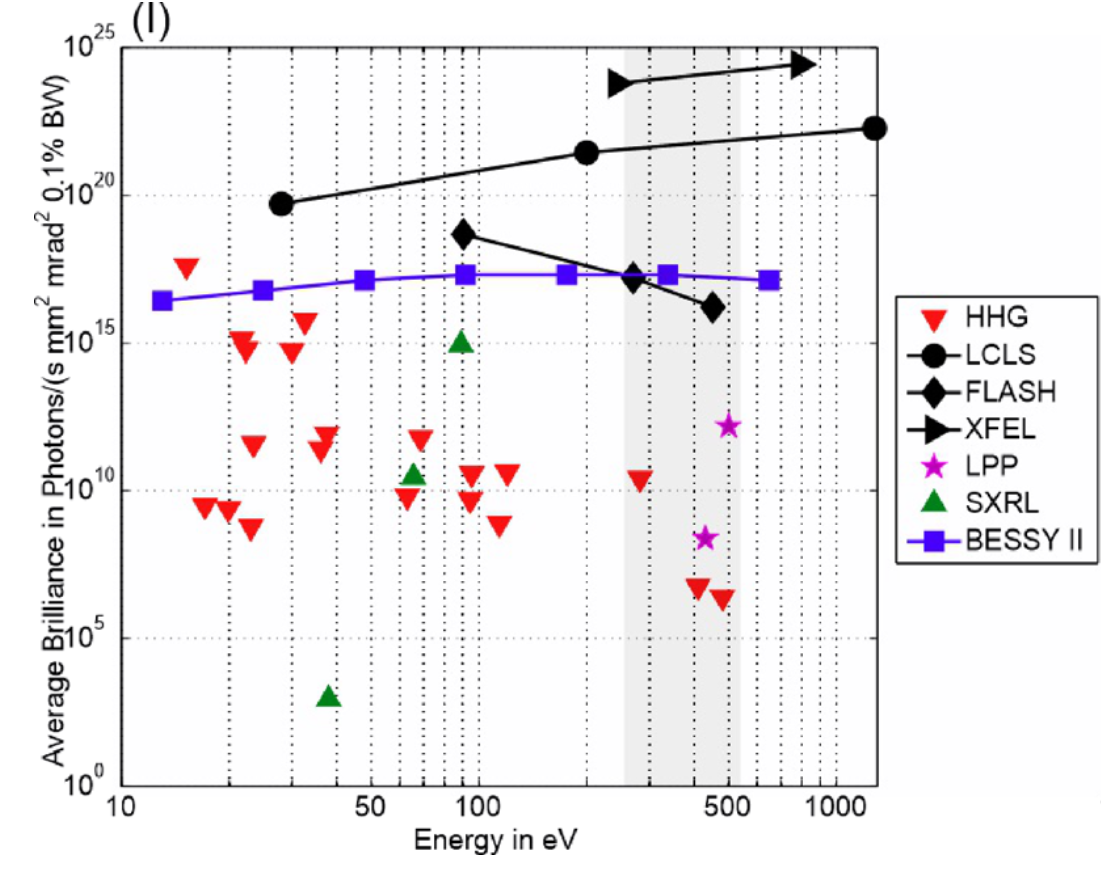
\includegraphics[width=0.9\linewidth]{Figures/XRaySourceBrilliance.png}
    \caption{Comparison of brightness as a function of 
        photon energy between conventional laser sources and higher 
        synchrotons, XFELs and harmonic generation sources, on a log-log scale. 
        \cite{Boutet2018}.
    }
    \label{fig:brilliance}
\end{figure}

\begin{figure}[h]
    \centering
    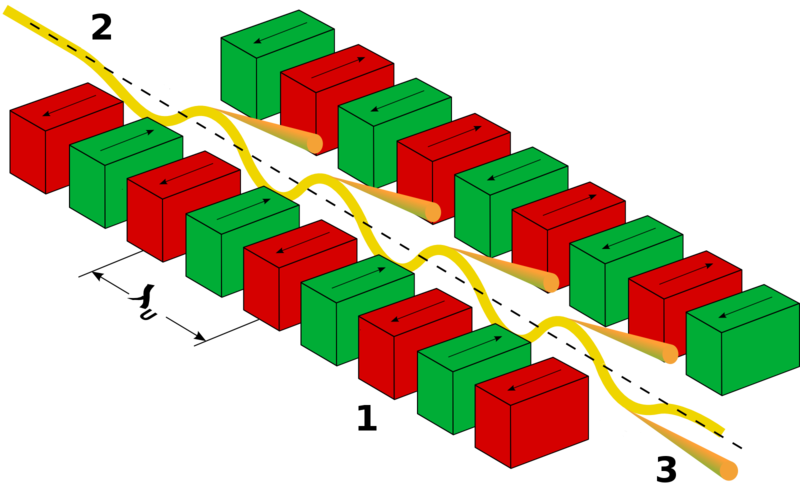
\includegraphics[width=0.9\linewidth]{Figures/800px-Undulator.png}
    \caption{Undulator schematic. Pictured are (1) two rows of adjacent magnets 
        of opposing polarities with spacing $\lambda_u/2$, (2) incident beam of
        electrons and (3) emitted radiation.}
    \label{fig:Undulator}
\end{figure}

%% TODO: Electron gun?

\subsection{Linear Accelerators}
XFELs and synchrotrons operate in a similar manner, accelerating electrons to
relativistic speeds and inducing synchrotron radiation via the Lorentz force.
Synchrotrons use bending magnets to curve the electron beam's trajectory, while
XFELs use undulators installed at the end of a linear accelerator (LINAC) to
generate coherent X-rays, though some synchrotrons have also implemented
undulators as insertion devices. Both sources require that electron bunches be
accelerated under vacuum, where the air pressure is of the order of $10^{-9}$
Torr to prevent beam scattering and energy loss. An initial, naive concept for
accelerating charges to such speeds would be to upscale the parallel-plate
capacitor, building a large potential difference across the plates and thus
accelerating electrons. While such devices do exist, called Van De Graaff
accelerators, they suffer from being too unstable when scaled up to the level
required to meet current energy thresholds, discharging (dangerously!) with
surrounding air. Thus, modern linear accelerators make use of more
sophisticated technology in the form of radio-frequency (RF) cavities. These
work via radio frequency electromagnetic pulses (often in the GHz range) sent
from a generator via a waveguide into spheroidal resonant cells which together
form a cavity. These waves resonate in the various cells, forming standing
waves. The system is engineered such that any two neighbouring cells are
$180^\circ$ out of phase. Thus, through precise timing, an electron bunch can
be sent through the first cell during its forward-thrusting phase, and by the
time it reaches the next cell, the standing wave pattern inverts and this cell,
too, is forward thrusting. This repeats ad nauseum until the electrons are at
the desired velocity. Of course, adjacent cells must be of increasing length
towards the start of the LINAC, such that as electrons increase in velocity,
traversing longer distances in the same amount of time, the arrival of the
electrons to the new cells are still synchronized with the standing wave
pattern. Towards the end of the LINAC, where electrons are in the relativistic
regime, speed increases become negligible and this ceases to be the case. 

    In state-of-the art XFEL facilities, such as EuXFEL and LCLS-II, 
superconducting radio-frequency (SRF) cavities are in use (often 
Niobium-based), kept at approximately two degrees kelvin. With this,
dissipative losses due to heat induced by surface currents as a result of the
electromagnetic waves in the cavity are astonishingly low. Thish drastically
increases the resonator's quality factor, defined as the ratio of stored energy
to the energy lost per cycle. It is often said that had Galileo, being one of
the first to study mechanical resonance in a pendulum in the 17^{\text{th}}$
century, worked with such a resonator operating at 1 Hz, this very pendulum
would still be swinging with about half its original amplitude
\cite{helmholtzSRF}. Such a high quality resonator enables continuous-wave
operation, in which the RF field in the cavity is maintained at a steady 
amplitude for long periods of time. This allows for multiple bunches to be 
accelerated with little-to-no down-time. Thus, the repetition rate of the 
aforementioned facilities is in the millions of electron bunches per second. 
Many other facilities, lagging behind on the adoption of SRF technology, are 
undergoing upgrades in accelerator design to meet such repetition rate demands,
thus enabling ultrafast science.

\begin{figure}[h]
    \centering
    \includegraphics[width=0.9\linewidth]{Figures/RFAcc.png}
    \caption{Superconducting radio-frequency cavity schematic with supporting
    He cooling system and vacuum \cite{helmholtzSRF}.}
    \label{fig:SRF}
\end{figure}


\subsubsection{Undulators}
Undulators, as can be seen in fig \ref{fig:Undulator}, are 
arrays of magnets of periodically alternating polarities. As an electron enters
this array at velocity $\textbf{u} \approx c$, it undergoes synchrotron 
radiation due to the acceleration caused by the sinusoidal magnetic field. In
the electron's centre of mass frame, where the undulator approaches at speed
$-\textbf{u}$, the undulator transverse $\textbf{B}$ field becomes the
combination of a transverse $\textbf{B}$ field and a transverse $\textbf{E}$
field via the Lorentz boosts:
\begin{align}
\mathbf{E}'_{\parallel} &= \mathbf{E}_{\parallel}, \quad \mathbf{B}'_{\parallel} = \mathbf{B}_{\parallel} \\
\mathbf{E}'_{\perp} &= \gamma (\mathbf{E}_{\perp} - u \mathbf{B}_{\perp}) \\
\mathbf{B}'_{\perp} &= \gamma \left( \mathbf{B}_{\perp} + \frac{u}{c^2} \mathbf{E}_{\perp} \right)
\end{align}
where $\gamma = \frac{1}{\sqrt{1 - u^2/c^2}}$ . Since the undulator field in
the lab frame is purely magnetic ($\textbf{E} = 0$), the transverse field in
the electron's rest frame simplifies to $\mathbf{E}'_{\perp} = - \gamma u
\mathbf{B}_{\perp}$. In essence, the system looks like an electromagnetic wave
approaching the electron, which in-turn causes the electron to radiate photons
of equal wavelength. This wavelength is given by the undulator period
$\lambda_u$ corrected for length contractions ($\lambda = \lambda_u/\gamma$).
However, the transverse velocity $\textbf{u}_{\perp}$ induced by the undulator
field slightly modifies the electron’s velocity components. Since the Lorentz
force cannot perform work, the total kinetic energy remains unchanged, but
$\textbf{u}_{\perp}$ reduces the electron’s longitudinal velocity to values
below $\textbf{u}$. It can therefore be shown that the wavelength measured in 
the lab frame becomes

\begin{equation}\label{equation: XFEL wl}
    \lambda = \frac{\lambda_u}{2\gamma^2}\left(1 + \frac{K^2}{2} \right)
\end{equation}

where,

\begin{equation}
    K = \frac{eB_0\lambda_u}{2\pi m_e c}.
\end{equation}
is known as the deflection parameter and is equal to the maximum angular
excursion of the beam in units of $1/\gamma$. Any device having $K < 1$ is
known as an undulator, while one with $K \gg 1$ is called a wiggler
\cite{CERN}. This result is handy as it
entails that the emitted wavelength of an XFEL may be tuned by adjusting the
magnetic field strength. It also reveals how much 
energy is required to accelerate electrons to sufficient speeds such that 
X-rays are emitted. 
    
    In reality, XFELs emit light with a bandwidth $\Delta\lambda$ centered
around the wavelength given by equation \ref{equation: XFEL wl}. This is due
the fact that each of the $N_u$ oscillations of the electron's sinusoidal motion 
contributes a wave packet of finite duration. The total physical length of the
resulting wave train is thus $L_t = N_u\lambda_u$, which leads to a wave train
duration of $T_t \approx L_t/c = N_u\lambda_u/c$. Since the Fourier transform 
of a finite-length wave scales as $1/T_t$, the spectral width becomes

\begin{equation}
    \frac{\Delta\lambda}{\lambda} = \frac{1}{N_u},
\end{equation}\label{eq:spread}
or $1/mN_u$ for the $m^{th}$ harmonic \cite{CERN}.

\subsubsection{Microbunching and Self-Amplified Spontaneous Emission (SASE)}

In reality, it is not a single electron that is accelerated into the undulator,
but groups of them called bunches. A bunch of electrons will emit X-rays as it
passes through the undulator, but the radiation will be incoherent due to the
random phase of the electrons. 

\begin{figure}[h]
    \centering
    \includegraphics[width=0.9\linewidth]{Figures/Microbunching.png}
    \caption{Mechanism of microbunching in an XFEL. ($a$) shows the progressive
        formation of microbunches as the electrons pass through the undulator.
        ($b$) shows the initial waves emitted by the electrons, and ($c$) shows
        how the spacing between the microbunches is determined by the undulator
        period. Finally, ($d$) shows the how the intensity of the emitted X-rays
        scales as a function of distance in the undulator, until the saturation
        point is reached, corresponding to where the electrons are maximally 
        bunched \cite{EMMA}.}
    \label{fig:Undulator}
\end{figure}
However, as the electrons travel through the
undulator, the waves they emit via spontaneous emission will interfere with 
other electrons. This interference can lead to the formation of microbunches,
where, depending on the relative phase of the electrons, the emitted radiation
will either accelerate or decelerate the electrons. This leads to the formation
of microbunches, which are ostensibly planes of electrons that emit coherent
X-rays, each conveniently being separated in space by the undulator period
$\lambda_u$. This phenomenon is known as self-amplified spontaneous emission 
(SASE) \cite{Saldin2006}.
This correlated emission of X-rays leads to a significant increase in the intensity
of the emitted radiation, as the waves emitted by the electrons constructively
interfere. This is illustrated in Fig. \ref{fig:Undulator}. The intensity of the
radiation scales exponentially as a function of distance in the undulator, as described 
by the following functional form:
\begin{equation}
    I(z) = I_0\exp\left(\frac{z}{l_g}\right),
\end{equation}
where $I_0$ is the initial intensity of the radiation, $z$ is the distance in the
undulator, and $l_g$ is the gain length, which is the distance over which the
intensity of the radiation increases by a factor of $e$ \cite{Bonifacio}. When 
building an undulator system, this result informs the optimal length to achieve 
the maximal theoretical intensity, with lengths exceeding those which achieve saturation 
proving to be unnecessary and cost-ineffective.

    The advantages SASE has towards high peak brilliances can be understood by 
considering the total electric field produced by the bunch when each electron
has a random phase $\phi_i$. The total electric field produced is simply the
real component of the superposition of each individual wave,
\begin{equation}
    E_{tot} = \Re \left\{ E_0 e^{i\omega t}\sum_{i = 0}^N e^{i\phi_i} \right \}.
\end{equation}
The root-mean-square amplitude, describing the average power, is thus dependent
upon the sum of squares of unit phasors

\begin{equation}
    Z^2 = \left\langle \left|\sum_{i=0}^N e^{i\phi_i}\right|^2 \right\rangle =
    \left\langle \sum_{i=0}^N \sum_{j=0}^N e^{i(\phi_i - \phi_j)}
    \right\rangle.
\end{equation}
We can easily compute this sum by considering the $i \neq j$ off-diagonal
instances separately. When this holds, we are effectively summing over unit 
phasors of random orientations in the complex plane, and thus the ensemble 
average vanishes. Conversely, when $i = j$, the phases subtract to zero in the 
exponent and so the sum overall evaluates to $N$. Thus, we find that the 
average power of such a beam scales linearly with the number of electrons in
the bunch. Now, consider an electron bunch all radiating with identical phase
$\phi$. The total electric field is trivially a superposition of $N$ identical
waves, which immediately gives $E_{tot} = \Re \{ NE_0e^{i(\omega t + \phi)} \}$.
Squaring this quantity, to obtain the power, we see that this now scales by the 
\textit{square} of the number of electrons. Noting that this quantity is often
in the hundreds of \textit{millions} to \textit{billions}, we can appreciate
the striking influence coherence has in brilliance contrasts between 
synchrotrons versus other X-ray sources.


\subsubsection{Bunch Compressors}
XFELs can be used to emit ultra fast X-ray pulses. The duration of a pulse
directly corresponds to the time it takes for the entire electron bunch to 
cross a certain point along the linear accelerator. To acheive shorter pulses,
bunch compressors are used to reduce the length of a bunch. 
Compressing an electron bunch is nontrivial, as the individual particles 
naturally repel each other via the Coulomb interaction. In practice, bunch 
compression is achieved by sending the electron bunch through a magnetic chicane.
The chicane consists of a series of magnets that bend the electron bunch in a
controlled manner, such that lower energy particles are deflected at greater 
angles, and thus must cover more distance, while higher energy particles are
deflected less. A bunch is said to have a negative energy chirp if tail electrons 
have higher energy than head electrons. With a negative energy chirp, the tail
electrons deflect less than the head electrons, allowing them to catch up to 
the head electrons, compressing the bunch \cite{Hastings2020}.

This enables the emitted beam to reach femtosecond to sub-femtosecond 
time scales, thus allowing researchers to study the dynamics of both surface and
sub-surface phenomena at nanometer or even atomic scales, where time-resolved
experiments employing optical lasers, such as optical reflectometry,
interferometry, and spectroscopy, suffer from limited spatial resolution and a
lack of bulk sensitivity
\cite{randolph2024subpicosecondsurfacecorrelationsfemtosecond}.

\begin{figure}[h]
    \centering
    \includegraphics[width=0.9\linewidth]{Figures/MagneticChicane.jpg}
    \caption{Process of electron bunch compression via a magnetic chicane.
    A typical chicane will consist of four dipole magnets of alternating
    polarities, pictured as green boxes. The black line shows the trajectory of
    reference particles, with the red line showing the trajectory of particles
    with lower energy, which are deflected more, and in blue the particles of
    higher energy, which are deflected less \cite{Hastings2020}.}
    \label{fig:Undulator}
\end{figure}

\subsubsection{Synchrotrons}
Synchrotrons differ from XFELs in that they accelerate charged particles in a
circular trajectory using bending magnets. The strength of the magnetic field
must be synchronized with the particle's energy, as a greater Lorentz force is
required to maintain the desired curved path as the particle's velocity
increases. Due to this radial acceleration, the charged particles emit
electromagnetic radiation. However, unlike in XFELs, this emitted radiation is
largely incoherent. Synchrotron radiation has a broad spectrum, making it 
versatile in this sense. Some synchrotrons are called storage rings, as they
maintain a beam of constant velocity particles circulating in a closed loop. 
In these facilities, radio-frequency cavities are used to compensate for the 
energy loss of the particles as they lose energy due to synchrotron radiation. 
Some synchrotrons have linear accelerators that provide an initial energy boost
to the particles before they are injected into the storage ring.
The emitted radiation is then directed to the experimental stations, where it is
used for X-ray diffraction, spectroscopy, and imaging \cite{Wiedemann2004}.


\begin{figure}[h]
    \centering
    \includegraphics[width=0.9\linewidth]{Figures/Synchrotron Facility.jpg}
    \caption{Typical layout of a synchrotron facility. The linear accelerator
    (LINAC) is used to accelerate particles to high energies before they are
    injected into a booster ring. The booster ring then accelerates the
    particles to even higher energies before they are injected into the storage
    ring. The storage ring maintains a beam of particles circulating in a closed
    loop via bending magnets, where they emit synchrotron radiation. This
    radiation is then directed to the experimental hutch. Certain insertion 
    devices, which may include undulators or wigglers, are used to generate
    higher intensity X-rays \cite{Wiedemann2004}.}
    \label{fig:Undulator}
\end{figure}




\section{Data Acquisition and Analysis} \label{sec:data}
Data acquisition in XFEL experiments is a complex process that involves
detection of often ultra-fast X-ray pulses operating at high luminosities. The
detectors used in these experiments must have high temporal resolution to
capture the fast dynamics of the pulses, and a dynamic gain switching
architecture to cope with said luminosities, while also being equipped with the
ability to detect traditional laser light with wavelengths in the visible to
infrared region with lower luminosities, allowing for pump-probe experiments
(see Section \ref{sec:pump-probe}). Said experiments require precise timing
synchronization systems to ensure that the pump and probe signals are properly
correlated. This typically requires a chain of mode-locked oscillators,
pulse-stretchers and compressors, regenerative amplifiers and multi-pass
amplifiers \cite{Togashi2025}. For detection, the European XFEL, for example,
is outfitted with a Large Pixel Detector (LPD), constructed with 16 identical
supermodules, each outfitted with a Front-End-Module which provides readout and
control functions. Such a detector is expected to generate 10 Gb/s of processed
data for every one Megapixel of sensor area \cite{JCoughlan_2011}. It
additionally uses an Adaptive Gain Integrating Pixel Detector, which is a
hybrid detector with a 4.5 MHz frame rate, and a dynamic range capable of
single photon resolution all the way up to a thousand 12.4 keV (X-ray energy)
photons \cite{MEZZA2019162606}. Other common types of detectors used are
scintillation detectors, which convert X-rays into visible light, and
semiconductor detectors, which convert X-rays into electrical signals, and
charge coupled devices (CCDs). The
latter are more sensitive and have a higher dynamic range, making them ideal
for high-resolution studies. The data collected by the detectors is then
processed using computational methods.

\subsubsection{The Phase Problem}
In the study of crystals by X-ray diffraction, the first step toward unveiling
the atomic structure lies in the careful measurement of diffracted intensities.
The intensity $I(hkl)$ of each diffraction spot is directly proportional to the
square of the modulus of the complex-valued structure factor:
\begin{equation}
    I(hkl) \propto |F(hkl)|^2
\end{equation}
The structure factor $F(hkl)$ encodes how all atoms within a unit cell
contribute to scattering in a given direction. It is defined as:
\begin{equation}
    F(hkl) = \sum_j f_j e^{2\pi i(hx_j +ky_j + lz_j)}
\end{equation}
where the sum runs over all atoms $j$ in the unit cell. Here, $f_j$ is the
\textit{atomic scattering factor} of atom $j$, a measure of how strongly the
atom scatters incident X-rays. It depends upon the number of
electrons in the atom and the scattering angle, as more electrons yield greater
scattering power. The coordinates $(x_j, y_j, z_j)$ are the \textit{fractional
atomic coordinates}, specifying the position of atom $j$ within the unit cell
as a fraction of the unit cell lengths $a$, $b$, and $c$ along the
crystallographic axes. These positions, taken together, define the geometric
and chemical structure of the unit cell and hence determine the resulting
interference pattern observed in reciprocal space. This summation defines the
complex structure factor, whose magnitude determines the measured intensity,
while its phase, essential for structure reconstruction, remains
experimentally inaccessible. Though X-ray diffraction patterns yield rich
structural insight, it is cursed with a fundamental shortcoming known as the
\textit{Phase Problem}. Detectors record only the intensities of the diffracted
beams, proportional to the square of the amplitude of the scattered waves, yet
the phase of each wave is tragically lost in measurement. To fully determine a
crystal's internal structure, one must reconstruct the electron density
function, which denotes the real-space positions of electrons, and hence,
atoms. The electron density function is given by
\begin{equation}
    \rho(x, y, z) = \frac{1}{V} \sum_{hkl} |F_{hkl}| \cdot 
    e^{-2\pi i [h\frac{x}{a} + k\frac{y}{b} + l\frac{z}{c} - \phi_{hkl}]},
\end{equation}
which is the inverse Fourier transform of the reciprocal-space structure
factors. As we can see, phase information is essential for reconstructing the
real-space electron density, and hence the Phase Problem is a central challenge
in crystallography.


\subsection{The Patterson Method}
\label{sec:patterson}
The challenges associated with measuring the relative phases among the diffracted 
beams $\phi_{hkl}$ makes determining the atomic positions within the unit cell 
difficult. Thankfully, in 1934, A. L. Patterson proposed a method to solve this 
problem. He showed that the one could replace the structure factors and 
phases in the electron density with the squared amplitudes of the structure factors 
alone \cite{Patterson1934}. This is beneficial, as the squared amplitudes can 
be directly measured from the diffraction pattern, and thus  the phase problem 
in crystallography is avoided. The Patterson function is defined as:

\begin{equation}
    P(u, v, w) = \frac{1}{V} \sum_{hkl} |F_{hkl}|^2 e^{2\pi i [hu/a + kv/b + lw/c]}.
\end{equation}
One may recognize this as the Fourier transform of the electron density, save for 
the fact that the structure factors are squared. This is by consequence of the 
Wiener-Khinchin theorem, which states that the Fourier transform of an 
auto-correlation function yields the squared magnitude of the Fourier components
of the original function. In this case, the Fourier transform of the Patterson
function gives the squared structure factors, $|F_{hkl}|^2$, which are
directly measurable from diffraction experiments. In this instance, the
Patterson function is the Fourier transform of the electron density's
auto-correlation function
\begin{equation}
    P(u, v, w) = \int \rho(x, y, z) \rho(x + u, y + v, z + w) d^3\textbf{r}
\end{equation}
which describes how well $\rho(\textbf{r})$ correlates with a version of itself 
shifted by an amount $(u, v, w)$, in another words, a convolution with its 
mirror image. This symmetry is tied to intrinsic symmetry exhibited by crystals,
and it can be shown that if one finds a maximum of $P(u, v, w)$, then at some
point ($u_1, v_1, w_1$), then there are atoms (correspoding to maxima of
$\rho(\textbf{r})$) whose distance apart is given by the vector whose components
are $(u_1, v_1, w_1)$ \cite{Patterson1934}. The Patterson function displays a
large number of peaks, specifically, for a crystal formed by $N$ atoms in the
unit cell, $P(u, v, w)$ will have $N^2$ maxima, corresponding to all possible
interatomic vectors, including self-vectors (see Fig. \ref{fig:Patterson}). One
can use the peak positions to determine the ($x, y, z$) coordinates of the atoms
in the unit cell using symmetry operations, as was first demonstrated by David 
Harker in 1935 \cite{Harker1936}. These peaks, qualitatively, have a
wide profile, as the atoms in the unit cell are not exactly point-like. This may
result in overlap among peaks. The heights of the peaks are proportional to the
atomic number of the constituents of the unit cell, and thus heavier atoms will
dominate the Patterson map, making for clear landmarks in the image. This method 
is complimentary to Rietveld refinement, as it can help establish the theoretical 
model for which the refinement process fits the data to. It is also generally 
quicker and simpler to perform, but yields less insight as a result.


\begin{figure}[h]
    \centering
    \includegraphics[width=0.9\linewidth]{Figures/Patterson-Function-Representation-of-the-Patterson-function-of-a-crystal-with-three-3553421574.png}
    \caption{Typical Patterson map of a crystal with three atoms in the unit cell.
        The peaks are labelled with their corresponding interatomic vectors 
    }
    \label{fig:Patterson}
\end{figure}

\subsection{Rietveld Refinement}
Rietveld refinement is a computational method used to determine the crystal
structure of a material from XRD data. It is typically used for powder samples,
where multiple reflections take place. It involves comparing the experimental
diffraction pattern $I_i^{\text{obs}}$ with a theoretical one $I_i^{\text{calc}}$
generated from a proposed crystal structure. A general recipe for obtaining a 
theoretical model of a diffraction pattern is to model the diffraction peak 
positions, intensities, and shapes, taking into account background contributions.

Peak positions, as described in section \ref{sec:theory}, are determined according 
to Bragg's law. For example, the orthorhombic crystal system has angles which obey 

\begin{equation}
    \begin{split}
        2\theta_{hkl} &= 2\arcsin\left(\frac{\lambda}{2d_{hkl}}\right), \\
        \text{where } d_{hkl} &= \left(\frac{h^2}{a^2} + \frac{k^2}{b^2} + \frac{l^2}{c^2}\right)^{-1/2}.
    \end{split}
\end{equation}

Since the Miller indices $h, k, l$ are integers, the peak positions are discontinuous,
which properly models the observed peak behaviour.

\begin{table*}[]
\caption{Factors affecting different components of an X-ray diffraction pattern.}
\label{tab:DiffractionFactors}
\centering
\begin{tabular}{llll}
\hline
Pattern component & Crystal structure & Specimen property & Instrumental parameter \\ \hline
\multirow{4}{*}{Peak position}  
  & \textbf{Unit cell parameters} & \textit{Absorption} & \textbf{Radiation (wavelength)} \\
  & ($a, b, c, \alpha, \beta, \gamma$) & Porosity & \textit{Instrument/sample alignment} \\
  & & & Axial divergence of the beam \\ \hline
\multirow{3}{*}{Peak intensity}  
  & \textbf{Atomic parameters} & \textit{Preferred orientation} & Geometry and configuration \\
  & ($x, y, z, B, \text{etc.}$) & Absorption & \textbf{Radiation (Lorentz, polarization)} \\
  & & \textit{Porosity} &  \\ \hline
\multirow{3}{*}{Peak shape}  
  & \textit{Crystallinity} & \textit{Grain size} & \textbf{Radiation (spectral purity)} \\
  & Disorder & \textit{Strain} & \textbf{Geometry} \\
  & Defects & \textit{Stress} & \textbf{Beam conditioning} \\ \hline
\multicolumn{4}{l}{Key parameters are shown in \textbf{bold}. Parameters that may have a significant influence are shown in \textit{italics}.} \\ \hline
\end{tabular}
\end{table*}

The intensity of the diffracted X-rays is a function of the structure factor
which depends upon the atomic positions, the multiplicity of the $k$ 
reflection $m_k$, the temperature factor $B_n$, and the atomic form factor $f_n$.
The form factor $f_n$ is a measure of the scattering power of an atom in the sample,
and is dependent on the electron density, the scattering angle and the
scatterer. That is, X-ray form factors are different from neutron form factors,
or electron form factors.  For various techniques, these factors are often
tabulated in the \textit{international tables for crystallography}
\cite{ITC_VolC}, alongside the multiplicity factors $m_k$, which refer to the
number of equivalent reflections that arise due to a certain crystal class'
symmetries.  The temperature factor, also called the Debye-Waller factor, is a
measure of the thermal vibrations of the atoms in the crystal. It accounts for
the attenuation of scattered X-rays due to the thermal motion of the atoms
\cite{Girolami}. Other factors which affects peak intensities include the Lorentz 
polarization factor $L_k$, which accounts for the polarization of the incident
beam and preferred-orientation factors $P_{kj}$, which account for anisotropy in 
the orientation distribution of diffraction data, which is a formalism used to 
describe the texture of a material \cite{BINNS2022231}. A polar diagram can be 
seen in figure \ref{fig:PolarDiagram}, which plots diffraction intensity 
as a function of azimuthal angle and Bragg angle, clearly showing the 
importance of considering anisotropic diffraction properties when modelling.

\begin{figure}[h]
    \centering
    \includegraphics[width=0.9\linewidth]{Figures/PolarDiagram.png}
    \caption{Polar diagram of a rolled aluminium sheet for beverage cans
        \cite{WRIGHT2005221}. Polar diagrams are graphical representations
        of how X-ray diffraction intensities vary with crystal orientation.
        They are used to visualize preferred orientation, texture effects 
        and anisotropic diffraction properties.
    }
    \label{fig:PolarDiagram}
\end{figure}


The peak shape functions $S_j$ are often modelled as a convolution of functions
that account for broadening effects due to the instrumentation, wavelength
dispersion, as described in the treatment of Eq \ref{eq:spread}, and the
intrinsic properties of the sample. Common peak profiles include the Gaussian,
Lorentzian, and pseudo-Voigt profiles. Absorption factors $A_j$, which account
for the attenuation of the beam by the sample play a role in peak shapes as well. 
    Finally, the background is often modelled as a polynomial function in $2\theta$ 
of degree $N_b$ of the form
\begin{equation}
    \text{bkg}(2\theta_i) = \sum_{j=0}^{N_b} a_j(2\theta_i)^j.
\end{equation}

Putting all these together, the model for the diffraction pattern is given by:
\begin{equation}
    \begin{split}
        I_i^{calc} = S_F \sum_{j=1}^{N_p} \frac{\phi_j}{V_j^2} \sum_{k=1}^N L_k |F_{kj}|^2 \\
        \times S_j(2\theta_i - 2\theta_{kj}) P_{kj} A_j + \text{bkg}(2\theta_i)
    \end{split}
\end{equation}
where $S_F$ is the beam intensity, $\phi_j$ is the phase volume fraction, and
$V_j$ is the phase cell volume, which is relevant for multiphase samples such as
polycrystalline materials. $L_k$ is the Lorentz factor, $F_{kj}$ is the structure
factor, $S_j$ is the peak shape function, $P_{kj}$ is the polarization factor,
and $A_j$ is the absorption factor. Factors which should be considered when 
modeling diffraction peaks can be found in \ref{tab:DiffractionFactors}, which
is taken from Pecharsky and Zavalij \cite{pecharsky2005fundamentals}.

With the model in hand, the Rietveld refinement process involves adjusting the
parameters to minimize the weighted sum of squares via 

\begin{equation}
    \begin{split}
    WSS = \sum_{i=1}^N \left[ w_i(I_i^{\text{obs}} - I_i^{\text{calc}})\right]^2, \\
    \text{where } w_i = \frac{1}{\sqrt{I_i^{obs}}}.
    \end{split}
\end{equation}
Here, $N$ is the number of observed data points. The process is
iterative, and the parameters are adjusted until the theoretical pattern matches
the experimental one. R indices are used to quantify the goodness of fit, defined
as 

\begin{equation}
    R_{\text{wp}} = \sqrt{\frac{\sum_{i = 1}^N[w_i(I_i^{obs} - I_i^{calc})]^2}
            {\sum_{i=1}^N (w_iI_i^{obs})^2}}
\end{equation}
\begin{equation}
    R_{\text{exp}} = \sqrt{\frac{(N - P)}{\sum_{i=1}^N (w_iI_i^{obs})^2}}
\end{equation}  
where P is the number of refined parameters. The goodness of fit is taken to be 
$R_{\text{wp}}/R_{\text{exp}}$, with values less than 2 indicating a good fit 
\cite{Lutterotti_Rietveld}. 


\begin{figure}[h]
    \centering
    \includegraphics[width=0.9\linewidth]{Figures/Typical-Rietveld-refinement-plot-LaMnO3-with-observed-black-circles-calculated.png}
    \caption{Rietveld refinement plot of LaMnO$_3$ by 
        P. Touseef and S. Shaibal \cite{RietveldExample}. The
        black circles are the observed data and the red line is the calculated
        spectrum via Rietveld refinement. The veritcal bars are the Bragg
        peak positions and the blue line shows the residuals.}
    \label{fig:RefinementFit}
\end{figure}

Rietveld refinement has many uses, from determining sample purity via 
measureing phase fractions with high accuracy, to determining atomic positions,
occupancies, thermal parameters and strain effects. It works with both X-ray 
and neutron diffraction data allowing for complimentary structural analyses.
Unfortunately, these advantages come at the high cost of requiring a detailed 
model with multiple parameters. This complexity may lead to overfitting to 
the model, and the refinement process is often computationally expensive.
Furthermore, this method is hightly sensitive, requiring good data quality, 
and only works for crystalline samples which have predicatable Bragg peaks, 
lest the model be drastically revised.

Common software packages for this technique include FullProf, GSAS and Reitan.
These offer support for crystallographic information files (CIF), which are 
standard files used to package information about crystal models, such as atomic 
positions, unit cell parameters, thermal parameters and space group
symmetry. Such files for common materials are often available from online 
databases \cite{RODRIGUEZCARVAJAL199355}.





\section{Experimental Techniques}

\subsection{Serial Femtosecond Crystallography (SFX)}
Many challenges arise when trying to measure diffraction peaks for
nanocrystals. The main hurdle is radiation damage, as X-rays are simply too
damaging and alter the structure of the specimen under study, yielding poor
results. Cryogenic cooling of samples is often employed to reduce the rate of
reactions within a sample, enabling it to withstand a 30-50 times increase in
exposure \cite{owen2006experimental}. This solution, however, complicates the
sample preparation process, and can be undesirable if one wishes to study
biological samples, for example, whose characteristics are wildly altered when
cooled to this degree. XFELs offer an alternative. XFELs are capable of
firing femtosecond flashes of X-rays that are shorter in time than it takes for
atoms in the sample to move \cite{neutze2000potential}. This is colloquially
referred to as "diffraction before destruction". Do not let this phrase fool
you; this technique will obliterate the specimen under study, as the intensity
of such pulses are akin to concentrating the intensity of the Sun's rays upon 
the planet Earth directly onto this poor nanocrystal \cite{SophiaChen}.
The power of this technique comes from the fact that the pulses themselves are
so short in duration that the X-rays are diffracted faster than the radiation
damage has time to manifest.

\begin{figure}[h]
    \centering
    \includegraphics[width=0.9\linewidth]{Figures/TypicalSFX.png}
    \caption{Typical SFX experimental setup. A nozzle fires a liquid jet 
    containing nanocrystals into the interaction point and enormous amounts of 
    XRD images are generated. The EuXFEL pulse structure is shown. Boasting an 
    effective repetition rate of 1.1 MHz, enough pulses are generated to 
    meet the crystal orientation sampling requirements \cite{Rahmani2023}.}
        \label{fig:SFX}
\end{figure}

No longer is growing a large crystal out of a specimen a requirement for
studying its diffraction patterns. Instead, the specimen nanocrystal is studied
and destroyed in series with each X-ray sampling a different random
orientation, and with enough sampling, impressive information about its
structure is gleaned. This is often done suspended in solution, with the
crystals floating into the line of fire. 

An interesting case study for this method happened during the COVID-19
pandemic. The Linac Coherent Light Source (LCLS) awarded rapid access beamtime
for seven SARS-CoV-2-related experiments in 2020 and 2021. These experiments
aimed to obtain radiation damage-free protein structures at room temperature
under physiological conditions, a key ability afforded by SFX. One
notable study focused on the SARS-CoV-2 main protease (MPro), a critical target
for drug development. The research team, based at KOÇ University in Istanbul,
was the first to take advantage of this special beamtime call. They
successfully solved the structure of MPro using SFX at the macromolecular
femtosecond crystallography (MFX) instrument at LCLS. The team used the
high-speed data collection capabilities of the facility to
test nine different drug candidates. These experiments were performed using
micrometer-sized crystals, which required the precision of XFELs to study
without causing radiation damage. This study contributed to the ongoing effort
to identify potential inhibitors for COVID-19 treatment and resulted in a
peer-reviewed publication \cite{Botha2023}.



%% TODO: Maybe more things?
%% TODO: Find a paper showing the benefits of ML for data selection.

%% TODO: Talk about the liquidography paper.

\subsection{Single Particle Imaging (SPI)}
Single particle imaging is similar to SFX but opts to study specimen devoid of
a crystal lattice, such as proteins, viruses, or macromolecular complexes. This
alone significantly alters the process of phase retrieval. 
%%TODO: Phase retrieval? Fourier synthesis? oversampled diffraction?
Where SFX benefits from Fourier synthesis and known crystallographic
methods, SPI must fight to scrounge for phase information, which is lost

The phase problem haunt us again, and not even the Patterson method can save us.
Non crystalline samples are simply too noisy.

The scattering signals from this method are additionally faint in comparison to
bright Bragg peaks. Experimentally, too, this method takes the harder path, 
and requires isolated particles. High vacuum (typically $10^{-5}-10^{-6}$ mbar)
is maintained at the interaction point, which is at the intersection of the 
X-ray beams and the single particle falling free from aerosol injection or 
from being electrosprayed.
%% TODO: Find paper using electrospray


revolutionary for structural biology, particularly in cases where samples are
not well-ordered crystals, and thus the techniques discussed previously fail. A
prime example is single-particle imaging (SPI), where individual biomolecules
or nanoparticles are injected into the XFEL beam as a gas-phase stream. Each
femtosecond pulse scatters off a single particle before radiation damage
destroys it, capturing a diffraction pattern that can be used to reconstruct
its structure. By collecting and computationally aligning thousands or millions
of such diffraction snapshots, researchers can assemble a high-resolution 3D
model of the particle without requiring crystallization.



\subsubsection{Machine Learning and Data Management}
These techniques generate enormous amounts of data, as hundreds of thousands of
diffraction peaks can be required to properly reconstruct the crystal
structure, and among these images reside just as many images of absolutely
nothing, as most X-rays simply miss the target altogether. Advancements in
computer vision are proving to increase the efficiency of
such methods. One way such advancements can benefit this technique is by data
reduction through filtering out undesireable events, such as missed shots, from
the pool of results immediately. For example, Rahmani et al. outline a method
of data reduction for SFX experiments by employing the \textit{Features from
Accelerated Segment Test} (FAST), an efficient corner-detection algorithm
for computer vision, allowing for the identification of Bragg peaks,
combined with \textit{Binary Robust Independent Elementary Features}
(BRIEF), which is a state-of-the art description algorithm which takes as
input the detected corners from FAST and generates compact binary strings
from these keypoints using relative pixel intensity differences, thus
encoding key features. Taking these two methods together, and making the
corner-detection rotationally invariant, and scale invariant, we arrive at
the \textit{Oriented FAST and Rotated BREIF} (ORB) method
\cite{Rahmani2023}. Machine learning algorithms such as multilayer perceptrons 
can then be used to classify the images using the ORB descriptions according to
more nuanced categories such as weak hits, strong hits, background dominated
images, etc. Further, advancements in convolutional neural network architecture
has led to machine-learning driven crystal structure identification 
\cite{ziletti2018insightful}.

\subsection{Pump-Probe Experiments}\label{sec:pump-probe}
The impressive temporal resolution of this technology enables experimenters to 
dynamically interact with a sample via a precisely-timed laser pulse, say, in
the visible region, called a pump, then later take a snapshot at some desired
time interval using X-ray pulses, called the probe. By repeating this process
and altering the time delay between the pump and the probe, a given specimen's
response to the laser pulse can be measured at any point along the process.
With this, one can image molecules undergoing chemical reactions, phase
transitions, structural reformations, electronic dynamics and so much more, all
without being limited to measurements in thermal or chemical equilibrium.
This technique gets us closer to making movies of such phenomena directly from
data, and can further our understanding of complicated dynamic processes. An 
example of this technique is [SOMEONE] et. al. imaging gold nanoparticles 
melting. In this experiment, the pump laser served to heat gold nanoparticles
and the probe measured the phase transition dynamics of solids melting. Another 
example is [SOMEONELSE] et al. group studying photosynthetic compounds by
shining "sunlight" as their pump, and probing the specimen to better understand
the dynamics of photosynthesis.

\newpage
\section{References}
\bibliographystyle{apsrev4-2}
\bibliography{references}

\end{document}

